\documentclass[10pt,paper=letter]{scrartcl}
\usepackage[alttitle]{cjquines}

\begin{document}

\title{VCSMS PRIME}
\subtitle{Program for Inducing Mathematical Excellence}
\author{Final Exam}
\date{Answer Key and Solutions}

\maketitle
\setlength{\unitlength}{1in}
\begin{picture}(0,0)
  \put(5.5,0.5){\hbox{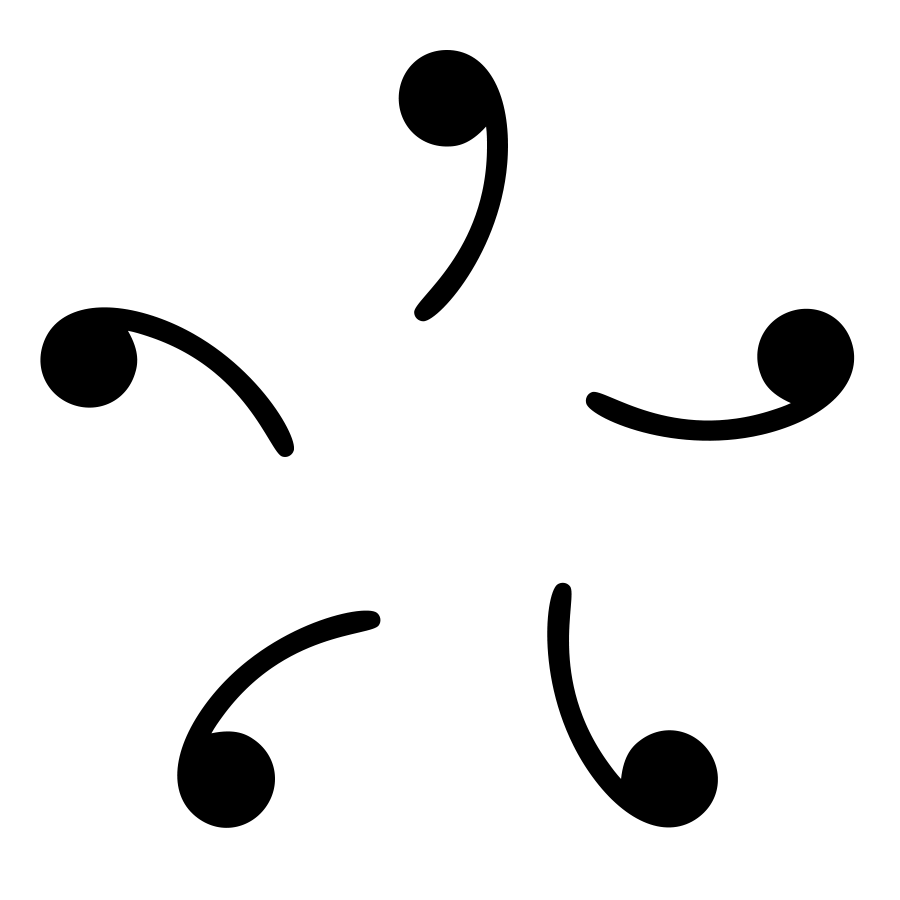
\includegraphics[width=0.9in]{logo.png}}}
\end{picture}
\vspace{-3em}

\begin{multicols}{3}
  \textbf{Part I. (2 points each)}
  \begin{enumerate}
    \item B
    \item C
    \item A
    \item A
    \item A
    \item A
    \item D
    \item A
    \item D
    \item B
    \item B
    \item C
    \item A
    \item C
    \item B
  \end{enumerate}
  \textbf{Part II. (3 points each)}
  \begin{enumerate}
    \item A
    \item B
    \item A
    \item B
    \item B
    \item C
    \item D
    \item B
    \item D
    \item D
  \end{enumerate}
  \textbf{Part III. (6 points each)}
  \begin{enumerate}
    \item 3531
    \item 13
    \item 1123
    \item $-3084$
    \item 239
  \end{enumerate}
\end{multicols}
\vspace{1em}

\noindent
\textbf{Disputes will be entertained for the first thirty minutes of lunch.} Afterward, scores in the finals and subsequently, grades in PRIME, will be finalized.

I have to acknowledge the contributions of Daniel, Sean, Dan, Ankan, Vinny, Weasley, Sharky and Kyle for providing comments on questions, correcting a few things, and test-solving.

\newpage

\subsubsection*{Part I}

\begin{enumerate}
  \item The choices are $121^6, 144^6, 125^6$ and $128^6$. The largest is B.
  \item Choice A is true because $5^2 + 5^2 > 6^2$, while $5^2 + 5^2 < 8^2$. Choice B is true because side $AB$ is the longest. The altitude from $C$ to $AB$ has length $4$ by the Pythagorean theorem, so $\tan \angle ABC = \frac43$, so C is false. Choice D is true because its perimeter is $6+5+5 = 16$ and its area is $4\cdot6/2 = 12$.
  \item Out of the $64$ possible outcomes, $\binom64$ have four heads, $\binom65$ have five heads and $\binom66$ has six heads. This makes a total of $22$ outcomes, so the probability is $11/32$.
  \item The giftees are split into cycles. Either there is one $6$-cycle, one $4$-cycle and one $2$-cycle, two $3$-cycles, or three $2$-cycles. The minimum number of moves needed to return nametags to their owners for each case are $6$, $4$, $3$ and $2$, respectively. The least common multiple is $12$.
  \item Triangle $PRO$ is isosceles, and $\angle PRO = 135\dg$ as it is an angle of a regular octagon. Thus $\angle POR = 22.5\dg$. Similarly, $\angle ANO = 108\dg$ as it is an angle of a regular pentagon, and from isosceles triangle $ANO$ we have $\angle AON = 36\dg$. Thus $\angle ROA = \angle PON - \angle POR - \angle AON = 108\dg - 22.5\dg - 36\dg = 49.5\dg$.
  \item Each of the choices are intervals of length $30$, which is $15\%$ of the maximum heart rate. The maximum heart rate must be $200$, so the interval needed is choice A.
  \item Square both sides and subtract $\sin^2 x + \cos^2 x = 1$ to get $\sin x \cos x = \dfrac7{18}$. Then $\sin^3 x + \cos^3 x = \del{\sin x + \cos x}^3 - 3(\sin x \cos x)(\sin x + \cos x) = \dfrac{22}{27}$.
  \item Each of the $a$ boys in Class A gets a female partner, and $x$ of the girls in Class B get a male partner. The remaining $b-x$ girls get a female partner. This is possible as $x < b$ and $a+b-x < y$. No larger assignment is possible.
  \item From $a^3 + b^3 + c^3 - 3abc = (a+b+c)(a^2 +b^2 +c^2 -ab -bc -ca)$, Vieta's gives $a^3 + b^3 + c^3 = 3abc = -51$.
  \item The ratio of the number of turns of two gears is the ratio of their radii. The ratios of the gears in between will cancel out, leaving only gears $A$ and $D$. Gear $A$ has radius $6$ and gear $D$ has radius $\sqrt{\dfrac6{\pi}}$. When gear $A$ is turned by $\dfrac{\pi}{2}$ radians, gear $D$ is turned by $\dfrac{\pi}2 \cdot \dfrac6{\sqrt{\frac6{\pi}}} = \dfrac{\pi\sqrt{6\pi}}2$ radians.
  \item The equations factor by SFFT as $(a+1)(b+2) = 15, (b+2)(c+3) = 42$ and $(c+3)(a+1) = 35$. Taking their product and the square root of both sides gives $(a+1)(b+2)(c+3) = 105\sqrt2$. Dividing the second equation gives $a = \dfrac{-2 + 5\sqrt2}2$, and the answer is $-2 + 5 + 2 + 2 = 7$.
  \item There are $5^5$ ways disregarding rotation. Subtract the $5$ colorings that are all the same color and divide by $5$ to get $5^4 - 1$ different colorings. Then add $5$ again to get $5^4 + 4$.
  \item We use the approximation $\sqrt{x-1} \approx \sqrt{x} - \dfrac1{2\sqrt{x}}$ from the binomial theorem or calculus. To the nearest hundredth, this is $26.20$. The actual value is about $26.176$.
  \item Choose the four couples to sit together in $\binom54$ ways. There are $4!$ ways to arrange them times $2^4$ ways, since each couple can switch. The two people in the remaining couple have to be separated; they can go in between or in the front and back. There are $7$ slots, so there are $\binom72$ ways times $2$, since they can switch. This is $80640$.
  \item Modulo $21$ this is $(-1)^{17} + \del{(-4)^6}^3\cdot(-4)^2 \equiv -1 + 1^3 \cdot 16 \equiv 15$.
\end{enumerate}

\subsubsection*{Part II}

\begin{enumerate}
  \item A number ending in $5$, when squared, ends in $25$; this makes $b = 2$. Thus the square of $\seg{ccc5}$ ends with $225$. We multiply out $c = 1$ to the fourth digit to rule it out. Same thing for $c = 2$, but only to the third digit. The first hit is $c = 3$, which gives $11122225$. 

  The other number of the form $\seg{aaa22225}$ differs from $11122225$ by a multiple of a large power of $10$. By difference of two squares, we want a number of the form $\seg{ccc5}$ to have sum with $3335$ that's divisible with a large power of $10$ as well. The only choice is $c = 6$, which gives $44422225$. Thus $1 + 4 = 5$.

  \emph{Alternatively}, one can use modulo $7$ and modulo $9$ to only retain $a = 1, 4, 7, 8$ as choices and use size arguments for $c$. 

  \item The radii of the circles are $\tan(\pi/4), \tan(\pi/8), \tan(\pi/16), \ldots$. The first is $1$, the second is $\sqrt2 - 1$. We approximate the rest using $\tan x \approx x$. This gives $$\pi + \pi\del{\sqrt2-1}^2 + \pi\del{\frac{\pi}{16}}^2 + \pi\del{\frac{\pi}{32}}^2 + \cdots = \del{1 + \del{3 - 2\sqrt2} + \frac{\frac{\pi^2}{256}}{1 - \frac14}}\pi,$$ by recognizing the rest of the terms as an infinite geometric series. Using $\pi^2 \approx 10$ and $\sqrt2 \approx 1.41$ gives to the hundredths place $1.23\pi$. The actual value is about $1.224\pi$.
  \item Let the centers be $A$ and $B$ and an intersection be $C$. Applying the law of cosines on $\angle ACB$ gives $AB^2 = AC^2 + BC^2 - 2\cdot AC\cdot BC\cdot\cos\angle ACB$, thus $\cos \angle ACB = \sqrt3/2$. Thus $\angle ACB = 30\dg$ and since $ABC$ is isosceles, $\angle CAB = \angle ABC = 75\dg$. The area is the area of two $150\dg$ sectors minus twice $[ABC]$. The former is $5\pi/3$, the latter is $1$.

  \item Point $X$ is closer to $A$ than $B$ if it lies on the side of the perpendicular bisector of $AB$ that contains $A$. This gives six inequalities, one for each of the $\binom42$ pairs of points. It is easier to plot the points in the plane and solve geometrically, as they lie on a triangular grid.

  Three of the inequalities cancel out: closer to $B$ than $D$, closer to $B$ than $C$, and closer to $A$ than $D$ are removed by both closer to $B$ than $C$ and closer to $C$ than $D$. The other boundary inequality is closer to $A$ than $B$. The intersection is a $30-60-90$ triangle with longer leg $1$. It thus has area $\frac{\sqrt3}{6}$.

  \item Since $6480 = 2^4 \cdot 3^4 \cdot 5$, note that the sum needed is $\del{1 - 2 + 2^2 - 2^3 + 2^4}\del{1 -3 + 3^2 - 3^3 + 3^4}\del{1-5}$ upon expanding. This evaluates to $-2684$.
  \item Let $\nu(x) = \nu_{2017}(x)$. Then $\nu\del{\binom{2017^2}{k}} = 2018 - \nu(k!) - \nu\del{(2017^2-k)!} = 2018 - \floor{\frac{k}{2017}} - \floor{\frac{2017^2 - k}{2017}}$. Writing $k = 2017n + d$, the valuation becomes $2018 - n - (2017 - n) = 1$, provided $0 < n < 2017$. This happens precisely when $1 \leq k \leq 2017^2 - 1$, giving $2017^2 - 1$ numbers.

  \emph{Alternatively}, one can look at Pascal's triangle and notice that all binomial coefficients on rows that are powers of primes are divisible by the prime.
  \item Well-known that polynomials in $\QQ[x]$ have the property that if $\sqrt{r}$ is a root for some rational $r$, then $-\sqrt{r}$ must be a root as well, thus $(x-\sqrt{r})(x+\sqrt{r}) = (x^2 - r)$ is a factor. In factored form, the polynomial must then be $2017^2\del{x^2 - \frac12}\del{x^2 - \frac13}\cdots\del{x^2 - \frac1{2017}}$. The sum of its coefficients is substituting $x = 1$, the product telescopes to $2017$.
  \item The numerator is $\log_n^2 \frac{n-1}{n^2}$ and the denominator is $\log_n^2 \del{2017 \cdot 2017!}$. By reverse change-of-base it simplifies to $\log_{2017 \cdot 2017!} \frac{n-1}{n^2}$. Applying the product rule gives $\log_{2017 \cdot 2017!} \frac1{2017 \cdot 2017!} = -1$.
  \item Let the foot from $C$ to $AB$ be $E$. Then $\triangle ABC$ is a $15-20-25$ right triangle, and by similarity the length of $AE$ is $16$ and the length of $CE$ is $12$. But the area of the isosceles trapezoid is $AE \times CE = 192$.

  \emph{Alternatively}, we can compute $CD = 7$ and use Brahmagupta's formula. 
  \item Recursion: either the leftmost is a vertical $1 \times 3$ rectangle or three horizontal $3 \times 1$ rectangles. If $f(n)$ is the number of ways to tile $3 \times n$ rectangle, then $f(n) = f(n-1) + f(n-3)$. We have $f(1) = f(2) = 1$ and $f(3) = 2$. From here, compute the rest of the sequence: $3, 4, 6, 9, 13, 19, 28, 41, 60, 88, 129, 189$.
\end{enumerate}

\subsubsection*{Part III}

\begin{enumerate}
  \item The largest among the ratios of digit value to matchsticks used is $7/4$, so it is optimal for Chris to keep making $7$s. He uses $2012$ of them to make $503$ $7$s. With the six remaining matchsticks he makes two $5$s, which is better than any other choice. This gives a total of $3531$.
  \item Let $[\mathcal{P}]$ be the area of polygon $\mathcal{P}$. Observe that $B$ and $C$ are the midpoints of $AA_B$ and $AA_C$, so $BC$ is half the length and parallel to $A_BA_C$, and thus $4[ABC] = [AA_BA_C]$. Thus $[BA_BA_CC] = 3[ABC]$. A similar argument holds for $[CB_CB_AA] = [AC_AC_BB] = 3[ABC]$.

  Then, $BA_B = BA$ and $BC_B = BC$ by reflection, also $\angle ABC = \angle A_BBC_B$ because they are vertical, it follows that triangles $ABC$ and $A_BBC_B$ are congruent. Thus $[A_BBC_B] = [ABC]$. Similarly, $[B_AAC_A] = [A_CCB_C] = [ABC]$. Finally, \begin{align*}[A_BA_CB_CB_AC_AC_B] &= [BA_BA_CC] + [CB_CB_AA] + [AC_AC_BB] \\ &+ [A_BBC_B] + [B_AAC_A] + [A_CCB_C] + [ABC] = 13[ABC],\end{align*} so the ratio needed is $13$.
  \item Let $\omega^3 = 1$ but $\omega \neq 1$. Then $\omega^2 + \omega + 1 = 0$. Substituting $\omega$ in $x^5 + x + 1$ gives $0$; it follows that $x^2 + x + 1$ is a factor of $x^5 + x + 1$. Thus $x^5 + x + 1 = (x^2 + x + 1)(x^3 - x^2 + 1)$.

  Thus $20^5 + 20 + 1 = (20^2 + 20 + 1)(20^3 - 20^2 + 1) = 421 \cdot 7601$. We observe that $7601$ is divisible by $11$; it is $11 \cdot 691$. We can verify by dividing small primes that $421$ and $691$ are both prime. The answer is $11 + 421 + 691 = 1123$.
  \item Multiply both sides by $xy$ and then substitute $x = a+b, y = a-b$. The condition becomes \begin{align*}
  y\sbr{f(x+y)+f(x-y)} - 4x^3y &= x\sbr{f(x+y)-f(x-y)} - 4xy^3\\
  (a-b)\sbr{f(2a)+f(2b)} - 4(a+b)^3(a-b) &= (a+b)\sbr{f(2a)-f(2b)} - 4(a+b)(a-b)^3\\
  2af(2b) + 16ab^3 &= 2bf(2a) + 16a^3b\\
  \frac{f(2b) + (2b)^3}{2b} &= \frac{f(2a) + (2a)^3}{2a}
  \end{align*}
  It follows that $\dfrac{f(x) + x^3}{x}$ is a constant for all $x$. Suppose it is $k$, then $f(x) = kx - x^3$. From $f(1) = 0$ we get $k=1$. Then $f(20) - f(17) = -3084$.

  \emph{Alternatively}, it is possible to substitute $(x, y) = (x, x), (-10, 10), (9, 8)$ to get $f(0), f(20)$ and $f(17)$.
  \item Represent as a string in base $2$: for example, $8$ would be $112$ and $81$ would be $121121$. For $f(n) = 3$, its string needs to have three $2$s. There are $\binom{3}{0}$ ways to have a string three characters long: $222$. There are $\binom{4}{1}$ ways to have a string four characters long, for $1222$, and so on. The sum is $\binom30 + \binom41 + \binom52 + \cdots$. This can be evaluated by the hockeystick identity, in particular the sum $\binom30 + \binom41 + \binom52 + \binom63 + \binom74 = 70$. The last string is thus $2221111$, or $239$.
\end{enumerate}

\newpage

\subsubsection*{Notes on test design}

A majority of the finals was produced over two weeks. Various problems were made beforehand from inspiration in everyday life, these were often the better ones. PMO 2016 was used as a reference for problem distribution: we all know PMO is heavily algebra-biased, but it is also biased towards geometry too. 

First, the target distribution of questions per topic per part was made, as well as a rough list of topics I wanted to appear. Existing questions were categorized and used initially; some had to be modified to be easier. Then I set out to write questions for the remaining topics. It was prepared concurrently with the solutions so as to make choice-writing easier.

Answers to the multiple choice part were generated with \url{random.org}. I also tried to sort answers in ``ascending'' order for some notion of ascending. This had the consequence of some problems having forced choices. Like II.1 had choice $17$ for the sum of two distinct digits, which only means $8+9$, which can then be easily eliminated.

Here's a breakdown. Part I:

\begin{enumerate}
  \item Number ripoff from 16QII7. The hard part was finding perfect powers that were near enough; there was an OEIS sequence for perfect powers so I used that.

  \item The idea of involving choices is pretty novel for PMO, the only reference on file being 16QI9. However, the inspiration comes from standardized testing questions like Regents, or the AMC. I also wanted to write a question that involved the triangle inequality, and ended up using a bunch of triangle concepts that I didn't use elsewhere. I don't think Heron's is a PMO quals topic, but it has appeared in areas.

  \item Standard fare. I needed a probability question, and was lacking easy questions, so I used this.

  The choice 1/2 and 21/32 were meant to trip people up; the latter was if it were at least three heads, not more than. The rest were written as in arithmetic sequence.

  \item I was trying to write an expected value question involving permutations. So the idea was like ``getting people to draw names from a hat'', and I was inspired by Secret Santa or Kris Kringle -- the way it worked was you gave to your giftee, then the giftee gives to theirs, and so on until it loops. I wanted to do an expected number of cycles, but ended up with this instead, which I think is nice for an easy question.

  The choices divisible by 5 were meant to trip up ``picks another person'' -- the permutation was a derangement. Then 144 was meant to trip up those who just multiplied. Nice fact that this also got LCM and casework out, which were also in my list of topics.

  \item Needed an angle chasing problem, the idea of regular polygons and their angles is standard fare. Polygon $PROBLEMS$ is stolen from HMMT or NIMO or something where it was $PROBLEMZ$. Then I needed another word, and I wanted to use a pentagon so I get weird angles. 

  Having $49.5\dg$ coming only from regular polygons and no arbitrary angles was very nice. Wanted a neat-looking angle in choices to trip up, so added $54\dg$ and did arithmetic sequence.

  \item I wrote this problem four months prior. This was inspired by a phys ed test I took in which I forgot the formula of maximum heart rate. Thankfully the choices were like this question, with intervals of the same size. Real life inspiration for the win; I think this problem is actually very nice.

  \item Standard fare. Wanted a trigonometry question that involved identities. This is very likely a number ripoff, but it was written independent of any particular problem as inspiration. 

  \item This problem was written two months prior. Originally the problem involved explicit numbers but I decided that was too easy. I needed an ``existence''-flavored combi problem.

  Inspiration from this came from those PIE-style problems like ``X do A, Y do B, max number of people who do both?'' and I wanted something else, so I thought of combining that idea with making partners.

  \item Wanted to use $a^3 + b^3 + c^3 = 3abc$ identity, which was disussed in PRIME. Sean commented that it was not a PMO quals topic, and I agreed, but it came up in class and was given emphasis.

  I was also thinking of writing a Vieta's problem, and wanted to do more than standard fare ``sum of reciprocals of roots''. So I was thinking sums of squares, sums of cubes -- and I remembered the identity. So I used that.

  Sean spotted an error (the choices were all positive originally) and got me to fix it, thanks.

  \item This was written one months prior. I was playing with an idea I saw from an old AusMC MP/UP: there was this small coin rolling around a big coin and the question was how many degrees it rolled. That got me thinking about gears, and turning gears.

  I filled in the details when I wrote the problem. Originally all the given were going to be radii of different sizes, but I thought of using diameters, etc. out of the blue. I didn't realize that the ratios telescoped, that was a nice touch. Choices were hoping for the common factor-of-two trip-up with radians.

  \item Needed a system of equations problem, and wanted to use the standard idea of ``add everything and divide by three''. But I needed variation. So I thought of making it a product. Then I thought of using SFFT like another prob. Then I realized I was ripping off 14NE4. Thanks to Sean for catching that $a, b, c$ can be negative.

  \item Needed an overcounting problem, so I thought of rotation. Did not want to make it full-blown Burnside's so I kept it prime. Choices were meant to trip people who just divided by five or missed a consideration.

  \item This is actually very naughty of me -- it is extremely unlikely that PMO will ever do an estimation question. But I wanted to, because MMC did anyway and we tackled it in class. Ankan liked this problem a lot for some reason.

  \item I needed a permutations problem and I wanted to involve stars and bars somehow. Permutation problem in mind, I thought of using couples. Then I realized, ``hey, I can turn this to a stars and bars type of problem''. So I did. Thanks to Sharky for choice-writing: factor-of-two and not separating the fifth couple.

  \item Standard fare. Needed a modulo problem, thought of using exponents which was pretty standard, and then thought of using the year. I was lacking standard problems in the test, so yeah.
\end{enumerate}

Part II. Sharky recommended the ordering seen here:

\begin{enumerate}
  \item This was actually the penultimate problem to be written. The original idea was trying to use bases: $\seg{abba}$ was a four-digit number which was a perfect cube in whatever base. That was too easy, so I tried again, still playing with the ideas of perfect powers in relation to bases.

  That lead to thinking of perfect powers in relation to digits, because I was considering divisibility by $11$ and palindromes and stuff. It was also because I noticed that $165^2 = 27225$ had particularly nice repeated digits. So I used a computer program to search for some powers with nice repeated digits.

  That lead to the beautiful $3335^2$ and $6665^2$. Originally the digit $5$ was meant to be a variable as well, but that was scrapped for being too hard. I thought of a relatively easy, though bashy solution. I showed this to a friend, asking for a non-bashy solution, and he gave two different ones and I really liked both.

  The $9$ choice was meant to trip up those who added the two possible values for $c$, the rest was arithmetic sequence.

  \item This was written two months ago. You know that AIME problem I think that involved a bunch of areas of circles in a triangle being in a geometric series? I wanted to do something like that as well. I was thinking about the golden spiral and this was kinda the same idea.

  Originally this was supposed to be about bounding the area with the difference of one large and one small circle, but I realized using trigonometry was easier. The series did not have an exact sum, so I used an approximation.

  This was, again, against the spirit of PMO to not use estimation problems, but I explicitly taught the technique in PRIME and the idea was nice.

  The choices used to be tighter than this, with differences of $0.02\pi$. But I wanted to not make accurate approximation a main point of the problem. Thanks to Sharky and Dan for phrasing issues.

  \item This was written two months ago. I was playing with the concept of area being pieced together and remembered the standard fare question of area between two circles passing through each others' centers. Then I thought of placing the circles together to make the angle different.

  This meant using trigonometry if I didn't make the angles explicit. I didn't want to use a standard sector angle, so I thought of $75\dg$. I was reminded of a trick I saw which splits a $15-75-90$ triangle to one $15-15-150$ triangle and one $30-60-90$ triangle, so that gave a nice non-trig way. 

  The numbers totally worked out in my head while I was walking home. I wrote it up and saved it. Then I revisited this problem and the numbers were all wrong. And then I realized that having $75\dg$ as an angle meant having $30\dg$, which made for a cleaner law of cosines solution. So I used that and some Wolfram Alpha to get some clean numbers. 

  \item Another question I wrote two months earlier. This was a ripoff from a Mathira 2017 question involving guessing the number of jellybeans, a one dimensional version of this problem. That one had a single possible number of jellybeans, and I ripped that problem off for a NIMO Revenge proposal that made it, which turned it to a range.

  Writing that problem made me think of solving the inequalities graphically. The idea of doing things graphically triggered a two-dimensional analogue, but I couldn't find pretty perpendicular bisectors. Then I thought of using a triangular grid and the problem popped out.

  One of the choices was in fact a mistake I made when solving this problem. I thought the answer was half the area of a unit equilateral triangle because of the triangular grid, but then it didn't match up with Geogebra. Whoops.

  \item Number ripoff from problem set by friend. I don't know how he came up with it, but it was a very good problem and I merely changed the numbers and the statement to make it neater. It was discrete Fourier analysis \emph{and} multiplicative number theory in a single problem! That was awesome.

  Choices are bad: one of them is sum of all the factors and the other two were negations.

  \item This was the last problem to be written, and thus pretty low-quality. Wanted to write a valuation problem, thought of binomial coefficients. I saw a theorem that about valuations of $p^n$ choose $k$ and thought of using a special case. This one was nice enough to be conjectured from smaller cases with Pascal's triangle, so yeah.

  Dan made the mistake of thinking $2017|k$, which inspired the choice $2017^2 - 2017$. The other two are OBOEs.

  \item This was one month earlier. I wanted to write a problem involving the minimal polynomial of $\sqrt{x}$. And then I also wanted to the factored form to have a telescoping product when substituting $P(k)$. I tried something more complicated but couldn't come up with anything good, so I was left with this.

  Thanks to Daniel and Vinny for some remarks. The choices are bad, I couldn't come up with anything.

  \item The idea, ``something telescoping with logs'', comes from about three months earlier, but the problem itself was one of the last to be written. Again, a telescoping product was turned to a sum. The idea was to make both the base and the argument things that were expanded out.

  The fact that the product of $(n-1)/n$ telescoped to $1/2017$ was boring -- I wanted to make the product more interesting. So I thought of squaring to make it a factorial, which meant the base was factorial as well, which fit with the idea of making the base expand. Then I just tried to write an expression that looked passable without being too complicated.

  Choices are bad.

  \item This is an idea from two months earlier, the same night as I came up with II.3. Observe that both play with the idea of area. This one was originally inspired by the fact that isosceles trapezoids are cyclic. I have no idea how I thought of combining that with right triangles, but their easily found altitude made the problem very nice.

  The nicer phrasing was ``an isosceles trapezoid has leg $15$, diagonal $20$ and base $25$'', but I opted on using more universal phrasing. The elegance of this problem lies on its statement.

  \item This was a very standard problem because I wanted a recursion problem and I couldn't make it too hard. I also couldn't come up with anything. That's why this problem is a number ripoff from an AusMC.
\end{enumerate}

Part III:

\begin{enumerate}
  \item The idea comes from two months earlier as well. I was thinking about 16AI20 and the sum of digits. I was also thinking about the recent NIMO Summer and the number of minutes per problem -- the ratio of points to minutes was a new idea for me. So I thought, how about the ratio of digits to something? But what?

  It had to be about building up digits. So the idea of segments on a seven-segment calculator came to mind first. Matchsticks made more natural phrasing. I thought of using $2017$ matchsticks, but I thought that making it $2018$ can allow one ot use the leftover matchstick to make $1$.

  Then the ratio $7/3$ was too big, so I thought of modifying the strict seven-segment to make $7$ have $4$ matchsticks. But then I realized that $7+1$ wasn't optimal for six matchsticks anymore, because $9$ was better! Playing on this idea lead to making $5$ have $3$ matchsticks instead.

  \item This comes way earlier -- the original idea was five months ago, was proof-based, and involved something extra, which I will withhold because it's nice. This modification of that problem is very nice because it has a very European-flavored dissection solution. 

  \item This is an evil problem. I was inspired by 16AI7 and $300^3 + 1$, which is apparently a ripoff of a common problem. I was thinking of a lot of algebraic factorizations, like Sophie--Germain and some other stuff, explicitly taught in PRIME.

  I eventually used $x^5 + x + 1$, when I factorized $10^5 + 10 + 1$ and $20^5 + 20 + 1$ and was satisfied with the latter as it only had three primes. It was good because one of them small and the other two easy to check for primality.

  \item This is an idea ripoff from Singaporean MO, with the sum and difference substitution and separating variables and getting the same expression on both sides. This is another one of those written backwards problems, and I was surprised I managed to get something which had a nice-ish statement. 

  Originally this would be III.5. Then a friend pointed out that one can get the answer without explicitly solving for $f$. I thought that was rather nice, and I kept it because it rewarded creativity -- though it made the problem easier, so I made it III.4. Sharky also commented that the combi problem should be last.

  \item Recall that earlier I wanted to write a problem about bases, and ended up with II.1. This was also an attempt to write a problem about bases. I was inspired by the numbers representable as sum of distinct powers of three, which turned to binary -- so I thought of other ways things can be turned to binary.

  I came up with this: changing binary from $0$s and $1$s to $1$s and $2$s, and using powers of two as the sum. Though, this made every number representable. So there went the ``find the 2017th smallest integer''.

  However, it made every number \emph{uniquely} representable. Which meant I can use properties of the representation itself. The obvious one was ``number of $2$s''. And when I started counting, I saw the sequence in OEIS -- apparently it's $\nu_2$ the $n$th Catalan number.

  Finding $f(n)$ for a given $n$ is easy. So I took the reverse approach: here's $f(n)$, find some $n$. Then I saw that it used combinatorial techniques, and that's when I reazlied this was a combi problem. It used hockeystick. The number $70$ was chosen because it gave an exact hockeystick sum, to make finding the original number easier.
\end{enumerate}

\end{document}
